%!TEX root = ../../msc17-game-book.tex

\phChapterWorksheet{Mummy Masquerade}{Main Puzzle 3}

Marvin Mummy has decided that this is finally the year he doesn't go as
himself for Halloween. And he's figured out the costume that will
finally make him the winner of Count
Calcula's annual costume contest. ``I'll dress up as \textit{Mummy Man},
the undead superhero with the power to wrap up crime!''

His lack of imagination aside, Marvin has at least decided to put a little
creativity into the design of his superbelt
(the source of Mummy Man's powers, duh!).

\begin{center}
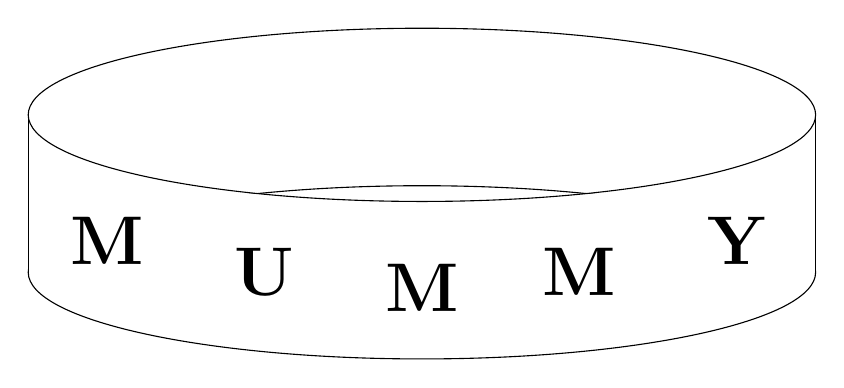
\begin{tikzpicture}
  \draw (0,0) ellipse (5 and 1.1);
  \fill[color=white] (-5,0) rectangle (5,1);
  \draw (-5,0) -- (-5,2);
  \draw (5,0) -- (5,2);
  \draw (0,2) ellipse (5 and 1.1);
  \node at (-4,0.4) {\Huge\bf M};
  \node at (-2,0) {\Huge\bf U};
  \node at (0,-0.2) {\Huge\bf M};
  \node at (2,0) {\Huge\bf M};
  \node at (4,0.4) {\Huge\bf Y};
\end{tikzpicture}
\end{center}

``I want curves
connecting each letter to each of the other letters, but I do NOT
want those curves to cross! They can go around or even behind on the back of the
belt, but I don't want the curve crossing another curve!''

Tape a strip of paper to make your own version of
Mummy Man's belt, writing the
letters M~U~M~M~Y anywhere you like. \textbf{How can you draw ten non-crossing
curves which connect each pair of letters?} Remember, these curves are allowed
to go around and behind the belt; actually, they'll have to!
